%%%%%%%%%%Packages%%%%%%%%%

\documentclass[11pt, titlepage, letterpaper, twoside]{article}
\usepackage{amsmath, amsthm, amssymb}
\usepackage{hyperref, pgf, tikz}
\usepackage{fancyhdr}
\usetikzlibrary{arrows}
\usepackage[margin=1.25in]{geometry}

%%%%%%%%%%%%%%%%%%%%%%%%%%%
\usetikzlibrary{circuits,circuits.ee.IEC}
\usepackage{circuitikz}
\tikzset{circuit declare symbol = amm}
\tikzset{set amm graphic ={draw,generic circle IEC, minimum size=7mm,info=center:A}}
\tikzset{circuit declare symbol = voltm}
\tikzset{set voltm graphic ={draw,generic circle IEC, minimum size=7mm,info=center:V}}


%%%%%%%%%%New Commands%%%%%%%%%



%%%%%%%%%%%%%%%%%%%%%%%%%%%
\pagestyle{fancy}
\frenchspacing

\lhead{Lab \#5 }  %insert lab # here
\rhead{\thepage}
\cfoot{}

\title{\textbf{RC Circuit with Oscilloscope} \\ \ \\ \large Lab \#5 }
\author{Name: Aidan Fitzgerald \\ Partners: Jason Shin, Victor Tan, and ???}
\date{June 7, 2016}
\begin{document}

\maketitle

\begin{center}
\LARGE RC Circuit with Oscilloscope
\end{center}

\section*{Objective}
Use an oscilloscope to observe the time constant of an RC circuit experimentally.

\section{Introduction}
Recall from Lab \#3 that the time constant $\tau$ of an RC circuit is the time during which the voltage
decays to $1/e \approx 37\%$ of its value. The time constant is equal to $RC$.

An analog oscilloscope is an electronic device that plots voltage as a function of time by deflecting
an electron beam in a cathode ray tube. In our setup it takes the place of a voltmeter.

\section{Procedures and Results}

We set up the circuit according to Figure 1, using an oscilloscope as a voltmeter and a function
generator in place of a battery.

\begin{figure}[h!]
  \centering
  \begin{circuitikz}[circuit ee IEC] \draw
    (0,0) to[R,l=$R$] (0,6) to[C,l=$C$] (6,6) to[voltm] (6,0) to[push button] (3,0) to[square voltage source,l=$V_0$] (0,0)
    ;
  \end{circuitikz}
  \caption{RC circuit}
\end{figure}

\pagebreak

We set the function generator to produce a square wave and observed an output signal that looked like a
series of spikes:

\begin{figure}[h!]
  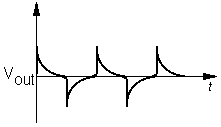
\includegraphics[scale=0.8]{rc_diff}
\end{figure}

We then set the function generator to produce a triangle wave and observed an output signal that
looked more like this:

\begin{figure}[h!]
  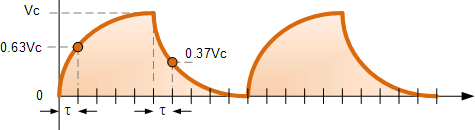
\includegraphics[scale=0.5]{rc_normal}
\end{figure}

\noindent which is more like the waveform we were told would appear. We adjusted the SEC/DIV knob of the
oscilloscope until the image was frozen on the screen and adjusted VOLTS/DIV so that the waveform
was 8 boxes high. Then, we measured the number of boxes across which the signal rose by 5 boxes.

\begin{table}[h!]
\centering
\caption{Oscilloscope measurements. Data courtesy of Margaret Burkart}
\label{observations}
\begin{tabular}{|l|l|l|l|l|}
\hline
Trial & Resistance       & Capacitance & Divisions across & SEC/DIV              \\ \hline
1     & $10,920\,\Omega$ & 900 pF      & 1.2              & $20\,\mathrm{\mu s}$ \\ \hline
2     & $5,555\,\Omega$  & 900 pF      & 1.9              & $20\,\mathrm{\mu s}$ \\ \hline
3     & $1,111\,\Omega$  & 900 pF      & 1.9              & $20\,\mathrm{\mu s}$ \\ \hline
4     & $5,555\,\Omega$  & 100 pF      & 1.8              & $20\,\mathrm{\mu s}$ \\ \hline
5     & $5,555\,\Omega$  & 500 pF      & 1.9              & $20\,\mathrm{\mu s}$ \\ \hline
\end{tabular}
\end{table}

\section{Discussion}

We calculated the observed time constant by multiplying the divisions across by the value of the SEC/DIV knob.
A sample calculation is shown for Trial 1:

$$
\tau_{observed} = 1.2 \times 20\,\mathrm{\mu s} = 24\,\mathrm{\mu s}
$$

We calculated an accepted value for $\tau$ by multiplying the resistance by the capacitance:

$$
\tau_{accepted} = 10,920\,\Omega \times 900\,\mathrm{pF} = 9.828\,\mathrm{\mu s}
$$

Then, we calculated the percent error:

$$
\mathrm{\%\,error} = \frac{\left| \tau_{observed} - \tau_{accepted} \right|}{\tau_{accepted}}
                   = \frac{\left| 24\,\mathrm{\mu s} - 9.828\,\mathrm{\mu s} \right|}{9.828\,\mathrm{\mu s}}
                   = 144 \%
$$

\begin{table}[h!]
\centering
\caption{Oscilloscope measurements. Data courtesy of Margaret Burkart}
\label{calculations}
\begin{tabular}{|l|l|l|l|}
\hline
Trial & $\tau_{observed}$    & $\tau_{accepted}$        & \% error \\ \hline
1     & $24\,\mathrm{\mu s}$ & $9.828\,\mathrm{\mu s}$  & 144 \%   \\ \hline
2     & $38\,\mathrm{\mu s}$ & $4.9995\,\mathrm{\mu s}$ & 660 \%   \\ \hline
3     & $38\,\mathrm{\mu s}$ & 999.9 ns                 & 3700\%   \\ \hline
4     & $36\,\mathrm{\mu s}$ & 555.5 ns                 & 6381\%   \\ \hline
5     & $38\,\mathrm{\mu s}$ & $2.7775\,\mathrm{\mu s}$ & 1268\%   \\ \hline
\end{tabular}
\end{table}


\section{Conclusion}
Today

\end{document}
